\documentclass[twoside]{book}

% Packages required by doxygen
\usepackage{fixltx2e}
\usepackage{calc}
\usepackage{doxygen}
\usepackage[export]{adjustbox} % also loads graphicx
\usepackage{graphicx}
\usepackage[utf8]{inputenc}
\usepackage{makeidx}
\usepackage{multicol}
\usepackage{multirow}
\PassOptionsToPackage{warn}{textcomp}
\usepackage{textcomp}
\usepackage[nointegrals]{wasysym}
\usepackage[table]{xcolor}

% Font selection
\usepackage[T1]{fontenc}
\usepackage[scaled=.90]{helvet}
\usepackage{courier}
\usepackage{amssymb}
\usepackage{sectsty}
\renewcommand{\familydefault}{\sfdefault}
\allsectionsfont{%
  \fontseries{bc}\selectfont%
  \color{darkgray}%
}
\renewcommand{\DoxyLabelFont}{%
  \fontseries{bc}\selectfont%
  \color{darkgray}%
}
\newcommand{\+}{\discretionary{\mbox{\scriptsize$\hookleftarrow$}}{}{}}

% Page & text layout
\usepackage{geometry}
\geometry{%
  a4paper,%
  top=2.5cm,%
  bottom=2.5cm,%
  left=2.5cm,%
  right=2.5cm%
}
\tolerance=750
\hfuzz=15pt
\hbadness=750
\setlength{\emergencystretch}{15pt}
\setlength{\parindent}{0cm}
\setlength{\parskip}{0.2cm}
\makeatletter
\renewcommand{\paragraph}{%
  \@startsection{paragraph}{4}{0ex}{-1.0ex}{1.0ex}{%
    \normalfont\normalsize\bfseries\SS@parafont%
  }%
}
\renewcommand{\subparagraph}{%
  \@startsection{subparagraph}{5}{0ex}{-1.0ex}{1.0ex}{%
    \normalfont\normalsize\bfseries\SS@subparafont%
  }%
}
\makeatother

% Headers & footers
\usepackage{fancyhdr}
\pagestyle{fancyplain}
\fancyhead[LE]{\fancyplain{}{\bfseries\thepage}}
\fancyhead[CE]{\fancyplain{}{}}
\fancyhead[RE]{\fancyplain{}{\bfseries\leftmark}}
\fancyhead[LO]{\fancyplain{}{\bfseries\rightmark}}
\fancyhead[CO]{\fancyplain{}{}}
\fancyhead[RO]{\fancyplain{}{\bfseries\thepage}}
\fancyfoot[LE]{\fancyplain{}{}}
\fancyfoot[CE]{\fancyplain{}{}}
\fancyfoot[RE]{\fancyplain{}{\bfseries\scriptsize Generated on Wed May 11 2016 18\+:45\+:13 for Practica5 by Doxygen }}
\fancyfoot[LO]{\fancyplain{}{\bfseries\scriptsize Generated on Wed May 11 2016 18\+:45\+:13 for Practica5 by Doxygen }}
\fancyfoot[CO]{\fancyplain{}{}}
\fancyfoot[RO]{\fancyplain{}{}}
\renewcommand{\footrulewidth}{0.4pt}
\renewcommand{\chaptermark}[1]{%
  \markboth{#1}{}%
}
\renewcommand{\sectionmark}[1]{%
  \markright{\thesection\ #1}%
}

% Indices & bibliography
\usepackage{natbib}
\usepackage[titles]{tocloft}
\setcounter{tocdepth}{3}
\setcounter{secnumdepth}{5}
\makeindex

% Hyperlinks (required, but should be loaded last)
\usepackage{ifpdf}
\ifpdf
  \usepackage[pdftex,pagebackref=true]{hyperref}
\else
  \usepackage[ps2pdf,pagebackref=true]{hyperref}
\fi
\hypersetup{%
  colorlinks=true,%
  linkcolor=blue,%
  citecolor=blue,%
  unicode%
}

% Custom commands
\newcommand{\clearemptydoublepage}{%
  \newpage{\pagestyle{empty}\cleardoublepage}%
}


%===== C O N T E N T S =====

\begin{document}

% Titlepage & ToC
\hypersetup{pageanchor=false,
             bookmarks=true,
             bookmarksnumbered=true,
             pdfencoding=unicode
            }
\pagenumbering{roman}
\begin{titlepage}
\vspace*{7cm}
\begin{center}%
{\Large Practica5 }\\
\vspace*{1cm}
{\large Generated by Doxygen 1.8.9.1}\\
\vspace*{0.5cm}
{\small Wed May 11 2016 18:45:13}\\
\end{center}
\end{titlepage}
\clearemptydoublepage
\tableofcontents
\clearemptydoublepage
\pagenumbering{arabic}
\hypersetup{pageanchor=true}

%--- Begin generated contents ---
\chapter{Hierarchical Index}
\section{Class Hierarchy}
This inheritance list is sorted roughly, but not completely, alphabetically\+:\begin{DoxyCompactList}
\item \contentsline{section}{Practica4.\+Arbitro}{\pageref{class_practica4_1_1_arbitro}}{}
\item \contentsline{section}{Practica4.\+Pelota}{\pageref{class_practica4_1_1_pelota}}{}
\item Runnable\begin{DoxyCompactList}
\item \contentsline{section}{Practica4.\+Jugador}{\pageref{class_practica4_1_1_jugador}}{}
\end{DoxyCompactList}
\end{DoxyCompactList}

\chapter{Class Index}
\section{Lista de clases}
Lista de las clases, estructuras, uniones e interfaces con una breve descripción\+:\begin{DoxyCompactList}
\item\contentsline{section}{\hyperlink{class_ejercicio1__3__3_1_1_detener___interrupcion}{Ejercicio1\+\_\+3\+\_\+3.\+Detener\+\_\+\+Interrupcion} \\*Thread que se detiene tras una señal del usuario, con diferentes acciones en función del tiempo transcurrido }{\pageref{class_ejercicio1__3__3_1_1_detener___interrupcion}}{}
\item\contentsline{section}{\hyperlink{class_ejercicio1__2__1_1_1_ejercicio1}{Ejercicio1\+\_\+2\+\_\+1.\+Ejercicio1} \\*Creación del número de hilos especificados por el usuario }{\pageref{class_ejercicio1__2__1_1_1_ejercicio1}}{}
\item\contentsline{section}{\hyperlink{class_ejercicio1__2__1_1_1_ejercicio2}{Ejercicio1\+\_\+2\+\_\+1.\+Ejercicio2} \\*Creación del número de hilos especificados por el usuario y medición del tiempo de ejecucion de los hilos }{\pageref{class_ejercicio1__2__1_1_1_ejercicio2}}{}
\item\contentsline{section}{\hyperlink{class_ejercicio1__2__4_1_1_ejercicio4}{Ejercicio1\+\_\+2\+\_\+4.\+Ejercicio4} \\*Cada thread calcula su tiempo de ejecución, lo almacena en una variable publica y se calcula el tiempo total }{\pageref{class_ejercicio1__2__4_1_1_ejercicio4}}{}
\item\contentsline{section}{\hyperlink{class_ejercicio1__2__5_1_1_ejercicio5}{Ejercicio1\+\_\+2\+\_\+5.\+Ejercicio5} \\*Muestra por separados los tiempos de inicialización de threads y los tiempos de ejecución de threads }{\pageref{class_ejercicio1__2__5_1_1_ejercicio5}}{}
\item\contentsline{section}{\hyperlink{class_ejercicio1__2__6_1_1_ejercicio6}{Ejercicio1\+\_\+2\+\_\+6.\+Ejercicio6} \\*Al crear los threads, en caso de introducir el valor \char`\"{}1\char`\"{} se realiza una operación compleja, en caso contrario se procede a la identificación finalización de los threads }{\pageref{class_ejercicio1__2__6_1_1_ejercicio6}}{}
\item\contentsline{section}{\hyperlink{class_ejercicio1__1__2_1_1hello_runnable}{Ejercicio1\+\_\+1\+\_\+2.\+hello\+Runnable} \\*Creación de hilos usando la clase Runnable }{\pageref{class_ejercicio1__1__2_1_1hello_runnable}}{}
\item\contentsline{section}{\hyperlink{class_ejercicio1__1__3_1_1hello_runnable___sleep}{Ejercicio1\+\_\+1\+\_\+3.\+hello\+Runnable\+\_\+\+Sleep} \\*Creación de hilos usando la clase Runnable y usando el método sleep para crear el delay de 1 segundo }{\pageref{class_ejercicio1__1__3_1_1hello_runnable___sleep}}{}
\item\contentsline{section}{\hyperlink{class_ejercicio1__1__2_1_1hello_thread}{Ejercicio1\+\_\+1\+\_\+2.\+hello\+Thread} \\*Creación de hilos usando la clase Thread }{\pageref{class_ejercicio1__1__2_1_1hello_thread}}{}
\item\contentsline{section}{\hyperlink{class_ejercicio1__1__3_1_1hello_thread___sleep}{Ejercicio1\+\_\+1\+\_\+3.\+hello\+Thread\+\_\+\+Sleep} \\*Creación de hilos usando la clase Thread y usando el método sleep para crear el delay de 1 segundo }{\pageref{class_ejercicio1__1__3_1_1hello_thread___sleep}}{}
\item\contentsline{section}{\hyperlink{class_ejercicio1__1__4_1_1_runnable___activo}{Ejercicio1\+\_\+1\+\_\+4.\+Runnable\+\_\+\+Activo} \\*Creación de hilos usando la clase Runnable y usando los metodos active\+Count y current\+Thread para postrar el numero de hilos y el hilo actual }{\pageref{class_ejercicio1__1__4_1_1_runnable___activo}}{}
\item\contentsline{section}{\hyperlink{class_ejercicio1__1__4_1_1_thread___activo}{Ejercicio1\+\_\+1\+\_\+4.\+Thread\+\_\+\+Activo} \\*Creación de hilos usando la clase Thread y usando los metodos active\+Count y current\+Thread para postrar el numero de hilos y el hilo actual }{\pageref{class_ejercicio1__1__4_1_1_thread___activo}}{}
\item\contentsline{section}{\hyperlink{class_ejercicio1__3__2_1_1_thread___detenido}{Ejercicio1\+\_\+3\+\_\+2.\+Thread\+\_\+\+Detenido} \\*Crea un Thread y comprueba con is\+Interrupted() e interrupted() antes y después de interrumpirlo }{\pageref{class_ejercicio1__3__2_1_1_thread___detenido}}{}
\end{DoxyCompactList}

\chapter{Class Documentation}
\hypertarget{class_client}{}\section{Client Class Reference}
\label{class_client}\index{Client@{Client}}


Clase que contiene el main del cliente que realiza la conexión y calcula \hyperlink{class_mandelbrot}{Mandelbrot}.  




Collaboration diagram for Client\+:
\nopagebreak
\begin{figure}[H]
\begin{center}
\leavevmode
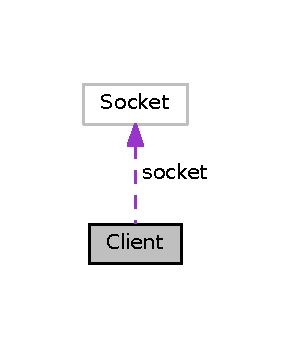
\includegraphics[width=140pt]{class_client__coll__graph}
\end{center}
\end{figure}
\subsection*{Static Public Member Functions}
\begin{DoxyCompactItemize}
\item 
static void \hyperlink{class_client_ab9b892ebe4b84667bfe6da7181385481}{main} (String\mbox{[}$\,$\mbox{]} args)  throws Class\+Not\+Found\+Exception, Interrupted\+Exception, I\+O\+Exception 
\begin{DoxyCompactList}\small\item\em Método main de la clase. \end{DoxyCompactList}\end{DoxyCompactItemize}
\subsection*{Static Protected Attributes}
\begin{DoxyCompactItemize}
\item 
\hypertarget{class_client_a8e8a6328d58ae78542f29ae058f2b909}{}static Socket {\bfseries socket}\label{class_client_a8e8a6328d58ae78542f29ae058f2b909}

\item 
\hypertarget{class_client_a6c6fb14b922f88c0ce93e9ee8b16478b}{}static Object\+Output\+Stream {\bfseries output}\label{class_client_a6c6fb14b922f88c0ce93e9ee8b16478b}

\item 
\hypertarget{class_client_a54dd9ac6c9b61f4c74977c17b20df71d}{}static Object\+Input\+Stream {\bfseries input}\label{class_client_a54dd9ac6c9b61f4c74977c17b20df71d}

\end{DoxyCompactItemize}


\subsection{Detailed Description}
Clase que contiene el main del cliente que realiza la conexión y calcula \hyperlink{class_mandelbrot}{Mandelbrot}. 

\begin{DoxyAuthor}{Author}
Nara, Javier, Esteban 
\end{DoxyAuthor}


\subsection{Member Function Documentation}
\hypertarget{class_client_ab9b892ebe4b84667bfe6da7181385481}{}\index{Client@{Client}!main@{main}}
\index{main@{main}!Client@{Client}}
\subsubsection[{main}]{\setlength{\rightskip}{0pt plus 5cm}static void Client.\+main (
\begin{DoxyParamCaption}
\item[{String\mbox{[}$\,$\mbox{]}}]{args}
\end{DoxyParamCaption}
) throws Class\+Not\+Found\+Exception, Interrupted\+Exception, I\+O\+Exception\hspace{0.3cm}{\ttfamily [static]}}\label{class_client_ab9b892ebe4b84667bfe6da7181385481}


Método main de la clase. 

\begin{DoxyAuthor}{Author}
Nara, Javier, Esteban 
\end{DoxyAuthor}

\begin{DoxyParams}{Parameters}
{\em args\mbox{[}$\,$\mbox{]}} & \+: Array de argumentos pasados como parámetros \\
\hline
\end{DoxyParams}


The documentation for this class was generated from the following file\+:\begin{DoxyCompactItemize}
\item 
Client.\+java\end{DoxyCompactItemize}

\hypertarget{class_complex}{}\section{Complex Class Reference}
\label{class_complex}\index{Complex@{Complex}}
\subsection*{Public Member Functions}
\begin{DoxyCompactItemize}
\item 
\hypertarget{class_complex_a6c6c07b34e6405445c264e11b47ccd43}{}{\bfseries Complex} (double real, double imag)\label{class_complex_a6c6c07b34e6405445c264e11b47ccd43}

\item 
\hypertarget{class_complex_a5a14ebec63aae370f2a05522e2c45453}{}String {\bfseries to\+String} ()\label{class_complex_a5a14ebec63aae370f2a05522e2c45453}

\item 
\hypertarget{class_complex_ad223eb3132189c3a0612249e78d337b5}{}double {\bfseries abs} ()\label{class_complex_ad223eb3132189c3a0612249e78d337b5}

\item 
\hypertarget{class_complex_a6c310c2a56601bf96ac682dd116fc8a0}{}double {\bfseries phase} ()\label{class_complex_a6c310c2a56601bf96ac682dd116fc8a0}

\item 
\hypertarget{class_complex_ac2c81dfbe734c25f94b2366ed451a986}{}\hyperlink{class_complex}{Complex} {\bfseries plus} (\hyperlink{class_complex}{Complex} b)\label{class_complex_ac2c81dfbe734c25f94b2366ed451a986}

\item 
\hypertarget{class_complex_afdf45232d33d711205be87bad5fae175}{}\hyperlink{class_complex}{Complex} {\bfseries minus} (\hyperlink{class_complex}{Complex} b)\label{class_complex_afdf45232d33d711205be87bad5fae175}

\item 
\hypertarget{class_complex_add864ec586b1fb6282b05197b7524617}{}\hyperlink{class_complex}{Complex} {\bfseries times} (\hyperlink{class_complex}{Complex} b)\label{class_complex_add864ec586b1fb6282b05197b7524617}

\item 
\hypertarget{class_complex_ab4b2c25339b9e0adb90380726877e42e}{}\hyperlink{class_complex}{Complex} {\bfseries times} (double alpha)\label{class_complex_ab4b2c25339b9e0adb90380726877e42e}

\item 
\hypertarget{class_complex_a6ac8c0c0e58c7c42563c3e850aa334eb}{}\hyperlink{class_complex}{Complex} {\bfseries conjugate} ()\label{class_complex_a6ac8c0c0e58c7c42563c3e850aa334eb}

\item 
\hypertarget{class_complex_a3abc78c5a8c36a75d16bd964e7e5cdca}{}\hyperlink{class_complex}{Complex} {\bfseries reciprocal} ()\label{class_complex_a3abc78c5a8c36a75d16bd964e7e5cdca}

\item 
\hypertarget{class_complex_a73bcffab86d38ffdced1219a19b8e417}{}double {\bfseries re} ()\label{class_complex_a73bcffab86d38ffdced1219a19b8e417}

\item 
\hypertarget{class_complex_a69879a11e4d8f26e7c9da46425976978}{}double {\bfseries im} ()\label{class_complex_a69879a11e4d8f26e7c9da46425976978}

\item 
\hypertarget{class_complex_ac102b0fa44b417c6ac84855ef18e3a42}{}\hyperlink{class_complex}{Complex} {\bfseries divides} (\hyperlink{class_complex}{Complex} b)\label{class_complex_ac102b0fa44b417c6ac84855ef18e3a42}

\item 
\hypertarget{class_complex_a0d1ea038cd8531bd25afd13e0ed370cc}{}\hyperlink{class_complex}{Complex} {\bfseries exp} ()\label{class_complex_a0d1ea038cd8531bd25afd13e0ed370cc}

\item 
\hypertarget{class_complex_a52fd914908413b162ea2840b711e3473}{}\hyperlink{class_complex}{Complex} {\bfseries sin} ()\label{class_complex_a52fd914908413b162ea2840b711e3473}

\item 
\hypertarget{class_complex_a3619fa0f81bf6d87888d13289232956b}{}\hyperlink{class_complex}{Complex} {\bfseries cos} ()\label{class_complex_a3619fa0f81bf6d87888d13289232956b}

\item 
\hypertarget{class_complex_a7efd64926947781a350971be3cc6337a}{}\hyperlink{class_complex}{Complex} {\bfseries tan} ()\label{class_complex_a7efd64926947781a350971be3cc6337a}

\end{DoxyCompactItemize}
\subsection*{Static Public Member Functions}
\begin{DoxyCompactItemize}
\item 
\hypertarget{class_complex_a93a5081483a5cad2da9f8bb6f9a1a6d1}{}static \hyperlink{class_complex}{Complex} {\bfseries plus} (\hyperlink{class_complex}{Complex} a, \hyperlink{class_complex}{Complex} b)\label{class_complex_a93a5081483a5cad2da9f8bb6f9a1a6d1}

\item 
\hypertarget{class_complex_a010780017cf90523d78217c89fe87d1e}{}static void {\bfseries main} (String\mbox{[}$\,$\mbox{]} args)\label{class_complex_a010780017cf90523d78217c89fe87d1e}

\end{DoxyCompactItemize}


The documentation for this class was generated from the following file\+:\begin{DoxyCompactItemize}
\item 
Complex.\+java\end{DoxyCompactItemize}

\hypertarget{class_data}{}\section{Data Class Reference}
\label{class_data}\index{Data@{Data}}


Clase que implementa los datos que se envían entre cliente y servidor.  




Inheritance diagram for Data\+:
\nopagebreak
\begin{figure}[H]
\begin{center}
\leavevmode
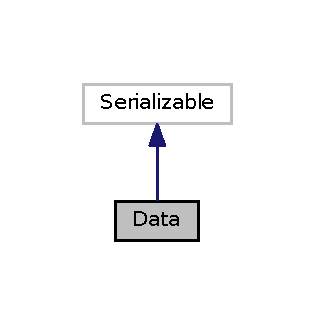
\includegraphics[width=151pt]{class_data__inherit__graph}
\end{center}
\end{figure}


Collaboration diagram for Data\+:
\nopagebreak
\begin{figure}[H]
\begin{center}
\leavevmode
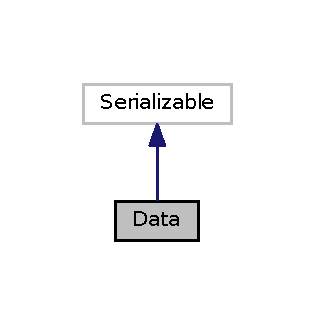
\includegraphics[width=151pt]{class_data__coll__graph}
\end{center}
\end{figure}
\subsection*{Public Member Functions}
\begin{DoxyCompactItemize}
\item 
\hyperlink{class_data_a4fd35b503a2759c5b67b30ae97efeabf}{Data} (String x, int s, int e, int it)
\begin{DoxyCompactList}\small\item\em Método constructor de la clase. \end{DoxyCompactList}\item 
void \hyperlink{class_data_a3677f709c98be676148e4fb8e08b1015}{set\+Datos\+Fractal} (double frac\+X, double frac\+Y, double s)
\begin{DoxyCompactList}\small\item\em Método que asigna los datos del fractal. \end{DoxyCompactList}\item 
void \hyperlink{class_data_ae26392ae0b534ed76ac0fe98d0b087fc}{set\+Picture} (Buffered\+Image p)
\begin{DoxyCompactList}\small\item\em Método que da valor a la imagen pic. \end{DoxyCompactList}\item 
Buffered\+Image \hyperlink{class_data_a64deecf379fc77a5c7fcc37524e793ba}{get\+Picture} ()
\begin{DoxyCompactList}\small\item\em Método que obtiene el valor de la imagen pic. \end{DoxyCompactList}\item 
int \hyperlink{class_data_a6bf2736c6dd62244dc1430723a3af3a7}{get\+N} ()
\begin{DoxyCompactList}\small\item\em Método que obtiene el número máxio de iteraciones. \end{DoxyCompactList}\item 
String \hyperlink{class_data_aabcc9cef01bd77c86ef0f67b09f95739}{get\+Accion} ()
\begin{DoxyCompactList}\small\item\em Método que obtiene la acción. \end{DoxyCompactList}\item 
void \hyperlink{class_data_a05f25af1300bdf02700165e8652f9fc7}{set\+Accion} (String x)
\begin{DoxyCompactList}\small\item\em Método que asigna una accion. \end{DoxyCompactList}\item 
double \hyperlink{class_data_a11f7bb2696a75bd529c384c8da242712}{get\+Size} ()
\begin{DoxyCompactList}\small\item\em Método que obtiene el tamaño de la imagen. \end{DoxyCompactList}\item 
void \hyperlink{class_data_a62cd79c3162b0695c7c37aabdb5566c6}{set\+Size} (double size)
\begin{DoxyCompactList}\small\item\em Método que asigna el tamaño de la imagen. \end{DoxyCompactList}\item 
int \hyperlink{class_data_a8f46b607e7967639d1ab96d429e4460c}{get\+Start} ()
\begin{DoxyCompactList}\small\item\em Método que obtiene la coordenada y de inicio. \end{DoxyCompactList}\item 
void \hyperlink{class_data_ad50db9eb7b9adc71e784ab67f9667efd}{set\+Start} (int start)
\begin{DoxyCompactList}\small\item\em Método que establece la coordenada Y donde inicia la iteracion. \end{DoxyCompactList}\item 
int \hyperlink{class_data_a98ee8be55a1ad0c2770ea852a19d738a}{get\+End} ()
\begin{DoxyCompactList}\small\item\em Método que obtiene la coordenada y de fin. \end{DoxyCompactList}\item 
void \hyperlink{class_data_a3dafc712a106610b47b89f76fff084e9}{set\+End\+End} (int end)
\begin{DoxyCompactList}\small\item\em Método que establece la coordenada Y donde termina la iteracion. \end{DoxyCompactList}\item 
void \hyperlink{class_data_a88f29c95fff497468476aa37093500fe}{set\+N} (int n)
\begin{DoxyCompactList}\small\item\em Método que asigna el numero máximo de iteraciones. \end{DoxyCompactList}\item 
double \hyperlink{class_data_ad5f6a3af2cf42e9ec692eeb46ec488c8}{get\+Fractal\+X} ()
\begin{DoxyCompactList}\small\item\em Método que obtiene el fractal en X. \end{DoxyCompactList}\item 
void \hyperlink{class_data_afb30418621a52ed2461dfe82e664fbaa}{set\+Fractal\+X} (double fractal\+X)
\begin{DoxyCompactList}\small\item\em Método que asigna el valor del fractal en X. \end{DoxyCompactList}\item 
double \hyperlink{class_data_a52eb15fc7662002f5d98e19dfbf0c735}{get\+Fractal\+Y} ()
\begin{DoxyCompactList}\small\item\em Método que obtiene el fractal en Y. \end{DoxyCompactList}\item 
void \hyperlink{class_data_a71af281cba7a7122e445d559aad231bf}{set\+Fractal\+Y} (double fractal\+Y)
\begin{DoxyCompactList}\small\item\em Método que asigna el valor del fractal en Y. \end{DoxyCompactList}\end{DoxyCompactItemize}


\subsection{Detailed Description}
Clase que implementa los datos que se envían entre cliente y servidor. 

\begin{DoxyAuthor}{Author}
Nara, Javier, Esteban 
\end{DoxyAuthor}


\subsection{Constructor \& Destructor Documentation}
\hypertarget{class_data_a4fd35b503a2759c5b67b30ae97efeabf}{}\index{Data@{Data}!Data@{Data}}
\index{Data@{Data}!Data@{Data}}
\subsubsection[{Data}]{\setlength{\rightskip}{0pt plus 5cm}Data.\+Data (
\begin{DoxyParamCaption}
\item[{String}]{x, }
\item[{int}]{s, }
\item[{int}]{e, }
\item[{int}]{it}
\end{DoxyParamCaption}
)}\label{class_data_a4fd35b503a2759c5b67b30ae97efeabf}


Método constructor de la clase. 

\begin{DoxyAuthor}{Author}
Nara, Javier, Esteban 
\end{DoxyAuthor}

\begin{DoxyParams}{Parameters}
{\em x} & \+: Nombre del paquete \\
\hline
{\em s} & \+: Coordenada Y del inicio de la iteración \\
\hline
{\em e} & \+: Coordenada Y del final de la iteración \\
\hline
{\em it} & \+: Número de iteraciones \\
\hline
\end{DoxyParams}


\subsection{Member Function Documentation}
\hypertarget{class_data_aabcc9cef01bd77c86ef0f67b09f95739}{}\index{Data@{Data}!get\+Accion@{get\+Accion}}
\index{get\+Accion@{get\+Accion}!Data@{Data}}
\subsubsection[{get\+Accion}]{\setlength{\rightskip}{0pt plus 5cm}String Data.\+get\+Accion (
\begin{DoxyParamCaption}
{}
\end{DoxyParamCaption}
)}\label{class_data_aabcc9cef01bd77c86ef0f67b09f95739}


Método que obtiene la acción. 

\begin{DoxyAuthor}{Author}
Nara, Javier, Esteban 
\end{DoxyAuthor}
\begin{DoxyReturn}{Returns}
accion \+: Número de jugadores del partido 
\end{DoxyReturn}
\hypertarget{class_data_a98ee8be55a1ad0c2770ea852a19d738a}{}\index{Data@{Data}!get\+End@{get\+End}}
\index{get\+End@{get\+End}!Data@{Data}}
\subsubsection[{get\+End}]{\setlength{\rightskip}{0pt plus 5cm}int Data.\+get\+End (
\begin{DoxyParamCaption}
{}
\end{DoxyParamCaption}
)}\label{class_data_a98ee8be55a1ad0c2770ea852a19d738a}


Método que obtiene la coordenada y de fin. 

\begin{DoxyAuthor}{Author}
Nara, Javier, Esteban 
\end{DoxyAuthor}
\begin{DoxyReturn}{Returns}
end \+: Coordenada Y donde termina la ieracion 
\end{DoxyReturn}
\hypertarget{class_data_ad5f6a3af2cf42e9ec692eeb46ec488c8}{}\index{Data@{Data}!get\+Fractal\+X@{get\+Fractal\+X}}
\index{get\+Fractal\+X@{get\+Fractal\+X}!Data@{Data}}
\subsubsection[{get\+Fractal\+X}]{\setlength{\rightskip}{0pt plus 5cm}double Data.\+get\+Fractal\+X (
\begin{DoxyParamCaption}
{}
\end{DoxyParamCaption}
)}\label{class_data_ad5f6a3af2cf42e9ec692eeb46ec488c8}


Método que obtiene el fractal en X. 

\begin{DoxyAuthor}{Author}
Nara, Javier, Esteban 
\end{DoxyAuthor}
\begin{DoxyReturn}{Returns}
fractal\+X \+: Fractal en X 
\end{DoxyReturn}
\hypertarget{class_data_a52eb15fc7662002f5d98e19dfbf0c735}{}\index{Data@{Data}!get\+Fractal\+Y@{get\+Fractal\+Y}}
\index{get\+Fractal\+Y@{get\+Fractal\+Y}!Data@{Data}}
\subsubsection[{get\+Fractal\+Y}]{\setlength{\rightskip}{0pt plus 5cm}double Data.\+get\+Fractal\+Y (
\begin{DoxyParamCaption}
{}
\end{DoxyParamCaption}
)}\label{class_data_a52eb15fc7662002f5d98e19dfbf0c735}


Método que obtiene el fractal en Y. 

\begin{DoxyAuthor}{Author}
Nara, Javier, Esteban 
\end{DoxyAuthor}
\begin{DoxyReturn}{Returns}
fractal\+X \+: Fractal en Y 
\end{DoxyReturn}
\hypertarget{class_data_a6bf2736c6dd62244dc1430723a3af3a7}{}\index{Data@{Data}!get\+N@{get\+N}}
\index{get\+N@{get\+N}!Data@{Data}}
\subsubsection[{get\+N}]{\setlength{\rightskip}{0pt plus 5cm}int Data.\+get\+N (
\begin{DoxyParamCaption}
{}
\end{DoxyParamCaption}
)}\label{class_data_a6bf2736c6dd62244dc1430723a3af3a7}


Método que obtiene el número máxio de iteraciones. 

\begin{DoxyAuthor}{Author}
Nara, Javier, Esteban 
\end{DoxyAuthor}
\begin{DoxyReturn}{Returns}
N \+: Número máximo de iteraciones 
\end{DoxyReturn}
\hypertarget{class_data_a64deecf379fc77a5c7fcc37524e793ba}{}\index{Data@{Data}!get\+Picture@{get\+Picture}}
\index{get\+Picture@{get\+Picture}!Data@{Data}}
\subsubsection[{get\+Picture}]{\setlength{\rightskip}{0pt plus 5cm}Buffered\+Image Data.\+get\+Picture (
\begin{DoxyParamCaption}
{}
\end{DoxyParamCaption}
)}\label{class_data_a64deecf379fc77a5c7fcc37524e793ba}


Método que obtiene el valor de la imagen pic. 

\begin{DoxyAuthor}{Author}
Nara, Javier, Esteban 
\end{DoxyAuthor}
\begin{DoxyReturn}{Returns}
pic \+: Valor de la imagen pic 
\end{DoxyReturn}
\hypertarget{class_data_a11f7bb2696a75bd529c384c8da242712}{}\index{Data@{Data}!get\+Size@{get\+Size}}
\index{get\+Size@{get\+Size}!Data@{Data}}
\subsubsection[{get\+Size}]{\setlength{\rightskip}{0pt plus 5cm}double Data.\+get\+Size (
\begin{DoxyParamCaption}
{}
\end{DoxyParamCaption}
)}\label{class_data_a11f7bb2696a75bd529c384c8da242712}


Método que obtiene el tamaño de la imagen. 

\begin{DoxyAuthor}{Author}
Nara, Javier, Esteban 
\end{DoxyAuthor}
\begin{DoxyReturn}{Returns}
size \+: Número de jugadores del partido 
\end{DoxyReturn}
\hypertarget{class_data_a8f46b607e7967639d1ab96d429e4460c}{}\index{Data@{Data}!get\+Start@{get\+Start}}
\index{get\+Start@{get\+Start}!Data@{Data}}
\subsubsection[{get\+Start}]{\setlength{\rightskip}{0pt plus 5cm}int Data.\+get\+Start (
\begin{DoxyParamCaption}
{}
\end{DoxyParamCaption}
)}\label{class_data_a8f46b607e7967639d1ab96d429e4460c}


Método que obtiene la coordenada y de inicio. 

\begin{DoxyAuthor}{Author}
Nara, Javier, Esteban 
\end{DoxyAuthor}
\begin{DoxyReturn}{Returns}
start \+: Coordenada Y donde inicia la ieracion 
\end{DoxyReturn}
\hypertarget{class_data_a05f25af1300bdf02700165e8652f9fc7}{}\index{Data@{Data}!set\+Accion@{set\+Accion}}
\index{set\+Accion@{set\+Accion}!Data@{Data}}
\subsubsection[{set\+Accion}]{\setlength{\rightskip}{0pt plus 5cm}void Data.\+set\+Accion (
\begin{DoxyParamCaption}
\item[{String}]{x}
\end{DoxyParamCaption}
)}\label{class_data_a05f25af1300bdf02700165e8652f9fc7}


Método que asigna una accion. 

\begin{DoxyAuthor}{Author}
Nara, Javier, Esteban 
\end{DoxyAuthor}

\begin{DoxyParams}{Parameters}
{\em jugadores} & \+: Acción a establecer \\
\hline
\end{DoxyParams}
\hypertarget{class_data_a3677f709c98be676148e4fb8e08b1015}{}\index{Data@{Data}!set\+Datos\+Fractal@{set\+Datos\+Fractal}}
\index{set\+Datos\+Fractal@{set\+Datos\+Fractal}!Data@{Data}}
\subsubsection[{set\+Datos\+Fractal}]{\setlength{\rightskip}{0pt plus 5cm}void Data.\+set\+Datos\+Fractal (
\begin{DoxyParamCaption}
\item[{double}]{frac\+X, }
\item[{double}]{frac\+Y, }
\item[{double}]{s}
\end{DoxyParamCaption}
)}\label{class_data_a3677f709c98be676148e4fb8e08b1015}


Método que asigna los datos del fractal. 

\begin{DoxyAuthor}{Author}
Nara, Javier, Esteban 
\end{DoxyAuthor}

\begin{DoxyParams}{Parameters}
{\em frac\+X} & \+: Número de jugadores del partido \\
\hline
{\em frac\+Y} & \+: Número de jugadores del partido \\
\hline
{\em s} & \+: Número de jugadores del partido \\
\hline
\end{DoxyParams}
\hypertarget{class_data_a3dafc712a106610b47b89f76fff084e9}{}\index{Data@{Data}!set\+End\+End@{set\+End\+End}}
\index{set\+End\+End@{set\+End\+End}!Data@{Data}}
\subsubsection[{set\+End\+End}]{\setlength{\rightskip}{0pt plus 5cm}void Data.\+set\+End\+End (
\begin{DoxyParamCaption}
\item[{int}]{end}
\end{DoxyParamCaption}
)}\label{class_data_a3dafc712a106610b47b89f76fff084e9}


Método que establece la coordenada Y donde termina la iteracion. 

\begin{DoxyAuthor}{Author}
Nara, Javier, Esteban 
\end{DoxyAuthor}

\begin{DoxyParams}{Parameters}
{\em start} & \+: Coordenada Y de fin \\
\hline
\end{DoxyParams}
\hypertarget{class_data_afb30418621a52ed2461dfe82e664fbaa}{}\index{Data@{Data}!set\+Fractal\+X@{set\+Fractal\+X}}
\index{set\+Fractal\+X@{set\+Fractal\+X}!Data@{Data}}
\subsubsection[{set\+Fractal\+X}]{\setlength{\rightskip}{0pt plus 5cm}void Data.\+set\+Fractal\+X (
\begin{DoxyParamCaption}
\item[{double}]{fractal\+X}
\end{DoxyParamCaption}
)}\label{class_data_afb30418621a52ed2461dfe82e664fbaa}


Método que asigna el valor del fractal en X. 

\begin{DoxyAuthor}{Author}
Nara, Javier, Esteban 
\end{DoxyAuthor}

\begin{DoxyParams}{Parameters}
{\em fractal\+X} & \+: Fractal en X \\
\hline
\end{DoxyParams}
\hypertarget{class_data_a71af281cba7a7122e445d559aad231bf}{}\index{Data@{Data}!set\+Fractal\+Y@{set\+Fractal\+Y}}
\index{set\+Fractal\+Y@{set\+Fractal\+Y}!Data@{Data}}
\subsubsection[{set\+Fractal\+Y}]{\setlength{\rightskip}{0pt plus 5cm}void Data.\+set\+Fractal\+Y (
\begin{DoxyParamCaption}
\item[{double}]{fractal\+Y}
\end{DoxyParamCaption}
)}\label{class_data_a71af281cba7a7122e445d559aad231bf}


Método que asigna el valor del fractal en Y. 

\begin{DoxyAuthor}{Author}
Nara, Javier, Esteban 
\end{DoxyAuthor}

\begin{DoxyParams}{Parameters}
{\em fractal\+X} & \+: Fractal en Y \\
\hline
\end{DoxyParams}
\hypertarget{class_data_a88f29c95fff497468476aa37093500fe}{}\index{Data@{Data}!set\+N@{set\+N}}
\index{set\+N@{set\+N}!Data@{Data}}
\subsubsection[{set\+N}]{\setlength{\rightskip}{0pt plus 5cm}void Data.\+set\+N (
\begin{DoxyParamCaption}
\item[{int}]{n}
\end{DoxyParamCaption}
)}\label{class_data_a88f29c95fff497468476aa37093500fe}


Método que asigna el numero máximo de iteraciones. 

\begin{DoxyAuthor}{Author}
Nara, Javier, Esteban 
\end{DoxyAuthor}

\begin{DoxyParams}{Parameters}
{\em n} & \+: Número máximo de iteraciones \\
\hline
\end{DoxyParams}
\hypertarget{class_data_ae26392ae0b534ed76ac0fe98d0b087fc}{}\index{Data@{Data}!set\+Picture@{set\+Picture}}
\index{set\+Picture@{set\+Picture}!Data@{Data}}
\subsubsection[{set\+Picture}]{\setlength{\rightskip}{0pt plus 5cm}void Data.\+set\+Picture (
\begin{DoxyParamCaption}
\item[{Buffered\+Image}]{p}
\end{DoxyParamCaption}
)}\label{class_data_ae26392ae0b534ed76ac0fe98d0b087fc}


Método que da valor a la imagen pic. 

\begin{DoxyAuthor}{Author}
Nara, Javier, Esteban 
\end{DoxyAuthor}

\begin{DoxyParams}{Parameters}
{\em p} & \+: Valor de la imagen \\
\hline
\end{DoxyParams}
\hypertarget{class_data_a62cd79c3162b0695c7c37aabdb5566c6}{}\index{Data@{Data}!set\+Size@{set\+Size}}
\index{set\+Size@{set\+Size}!Data@{Data}}
\subsubsection[{set\+Size}]{\setlength{\rightskip}{0pt plus 5cm}void Data.\+set\+Size (
\begin{DoxyParamCaption}
\item[{double}]{size}
\end{DoxyParamCaption}
)}\label{class_data_a62cd79c3162b0695c7c37aabdb5566c6}


Método que asigna el tamaño de la imagen. 

\begin{DoxyAuthor}{Author}
Nara, Javier, Esteban 
\end{DoxyAuthor}

\begin{DoxyParams}{Parameters}
{\em size} & \+: Tamaño de la imagen a establecer \\
\hline
\end{DoxyParams}
\hypertarget{class_data_ad50db9eb7b9adc71e784ab67f9667efd}{}\index{Data@{Data}!set\+Start@{set\+Start}}
\index{set\+Start@{set\+Start}!Data@{Data}}
\subsubsection[{set\+Start}]{\setlength{\rightskip}{0pt plus 5cm}void Data.\+set\+Start (
\begin{DoxyParamCaption}
\item[{int}]{start}
\end{DoxyParamCaption}
)}\label{class_data_ad50db9eb7b9adc71e784ab67f9667efd}


Método que establece la coordenada Y donde inicia la iteracion. 

\begin{DoxyAuthor}{Author}
Nara, Javier, Esteban 
\end{DoxyAuthor}

\begin{DoxyParams}{Parameters}
{\em start} & \+: Coordenada Y de inicio \\
\hline
\end{DoxyParams}


The documentation for this class was generated from the following file\+:\begin{DoxyCompactItemize}
\item 
Data.\+java\end{DoxyCompactItemize}

\hypertarget{class_iteration}{}\section{Iteration Class Reference}
\label{class_iteration}\index{Iteration@{Iteration}}
\subsection*{Public Member Functions}
\begin{DoxyCompactItemize}
\item 
\hypertarget{class_iteration_a3c8711e364f6e88b21ef01b091a205a0}{}{\bfseries Iteration} (int start, int end)\label{class_iteration_a3c8711e364f6e88b21ef01b091a205a0}

\end{DoxyCompactItemize}
\subsection*{Public Attributes}
\begin{DoxyCompactItemize}
\item 
\hypertarget{class_iteration_a485681615fc5cb63e99d7ce84f838a57}{}int {\bfseries start}\label{class_iteration_a485681615fc5cb63e99d7ce84f838a57}

\item 
\hypertarget{class_iteration_a771e1a72b8aec943d69fe53eea78d956}{}int {\bfseries end}\label{class_iteration_a771e1a72b8aec943d69fe53eea78d956}

\end{DoxyCompactItemize}


The documentation for this class was generated from the following file\+:\begin{DoxyCompactItemize}
\item 
Iteration.\+java\end{DoxyCompactItemize}

\hypertarget{class_mandelbrot}{}\section{Mandelbrot Class Reference}
\label{class_mandelbrot}\index{Mandelbrot@{Mandelbrot}}


Clase que realiza el cálculo de \hyperlink{class_mandelbrot}{Mandelbrot}.  




Collaboration diagram for Mandelbrot\+:
\nopagebreak
\begin{figure}[H]
\begin{center}
\leavevmode
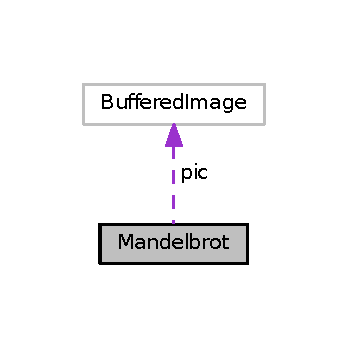
\includegraphics[width=167pt]{class_mandelbrot__coll__graph}
\end{center}
\end{figure}
\subsection*{Public Member Functions}
\begin{DoxyCompactItemize}
\item 
\hyperlink{class_mandelbrot_a09830bd77bc96c054e4e453e8326fda1}{Mandelbrot} (double x, double y, double s, int n, int m, int iterations)
\begin{DoxyCompactList}\small\item\em Método constructor de la clase. \end{DoxyCompactList}\item 
Buffered\+Image \hyperlink{class_mandelbrot_a51a2075937f0553564a5040f44070500}{realizar\+Fractal} (int start, int end, int width)
\begin{DoxyCompactList}\small\item\em Método que crea el fractal. \end{DoxyCompactList}\end{DoxyCompactItemize}
\subsection*{Static Public Member Functions}
\begin{DoxyCompactItemize}
\item 
static int \hyperlink{class_mandelbrot_a5f0b4399e850a94193d87e03cca38736}{mand} (\hyperlink{class_complex}{Complex} z0, int max)
\begin{DoxyCompactList}\small\item\em Método que realiza el cálculo de Nabdekbrot. \end{DoxyCompactList}\end{DoxyCompactItemize}


\subsection{Detailed Description}
Clase que realiza el cálculo de \hyperlink{class_mandelbrot}{Mandelbrot}. 

\begin{DoxyAuthor}{Author}
Nara, Javier, Esteban 
\end{DoxyAuthor}


\subsection{Constructor \& Destructor Documentation}
\hypertarget{class_mandelbrot_a09830bd77bc96c054e4e453e8326fda1}{}\index{Mandelbrot@{Mandelbrot}!Mandelbrot@{Mandelbrot}}
\index{Mandelbrot@{Mandelbrot}!Mandelbrot@{Mandelbrot}}
\subsubsection[{Mandelbrot}]{\setlength{\rightskip}{0pt plus 5cm}Mandelbrot.\+Mandelbrot (
\begin{DoxyParamCaption}
\item[{double}]{x, }
\item[{double}]{y, }
\item[{double}]{s, }
\item[{int}]{n, }
\item[{int}]{m, }
\item[{int}]{iterations}
\end{DoxyParamCaption}
)}\label{class_mandelbrot_a09830bd77bc96c054e4e453e8326fda1}


Método constructor de la clase. 

\begin{DoxyAuthor}{Author}
Nara, Javier, Esteban 
\end{DoxyAuthor}

\begin{DoxyParams}{Parameters}
{\em x} & \+: Valor de x \\
\hline
{\em y} & \+: Valor de y \\
\hline
{\em s} & \+: Tamaño de la iteración \\
\hline
{\em n} & \+: Tamaño de los lados de la imagen \\
\hline
{\em m} & \+: Número máximo de iteraciones \\
\hline
{\em iterations} & \+: Número de iteraciones \\
\hline
\end{DoxyParams}


\subsection{Member Function Documentation}
\hypertarget{class_mandelbrot_a5f0b4399e850a94193d87e03cca38736}{}\index{Mandelbrot@{Mandelbrot}!mand@{mand}}
\index{mand@{mand}!Mandelbrot@{Mandelbrot}}
\subsubsection[{mand}]{\setlength{\rightskip}{0pt plus 5cm}static int Mandelbrot.\+mand (
\begin{DoxyParamCaption}
\item[{{\bf Complex}}]{z0, }
\item[{int}]{max}
\end{DoxyParamCaption}
)\hspace{0.3cm}{\ttfamily [static]}}\label{class_mandelbrot_a5f0b4399e850a94193d87e03cca38736}


Método que realiza el cálculo de Nabdekbrot. 

\begin{DoxyAuthor}{Author}
Nara, Javier, Esteban 
\end{DoxyAuthor}

\begin{DoxyParams}{Parameters}
{\em z0} & \+: Número complejo para realizar el cálculo \\
\hline
{\em max} & \+: Número máximo de iteraciones \\
\hline
\end{DoxyParams}
\begin{DoxyReturn}{Returns}
max \+: Nuevo Número máximo de iteraciones 
\end{DoxyReturn}
\hypertarget{class_mandelbrot_a51a2075937f0553564a5040f44070500}{}\index{Mandelbrot@{Mandelbrot}!realizar\+Fractal@{realizar\+Fractal}}
\index{realizar\+Fractal@{realizar\+Fractal}!Mandelbrot@{Mandelbrot}}
\subsubsection[{realizar\+Fractal}]{\setlength{\rightskip}{0pt plus 5cm}Buffered\+Image Mandelbrot.\+realizar\+Fractal (
\begin{DoxyParamCaption}
\item[{int}]{start, }
\item[{int}]{end, }
\item[{int}]{width}
\end{DoxyParamCaption}
)}\label{class_mandelbrot_a51a2075937f0553564a5040f44070500}


Método que crea el fractal. 

\begin{DoxyAuthor}{Author}
Nara, Javier, Esteban 
\end{DoxyAuthor}

\begin{DoxyParams}{Parameters}
{\em start} & \+: Coordenada Y donde comienza la Iteracion \\
\hline
{\em end} & \+: Coordenada Y donde acaba la Iteracion \\
\hline
{\em width} & \+: Ancho total de la imagen de la Iteración \\
\hline
\end{DoxyParams}
\begin{DoxyReturn}{Returns}
\+: Imagen pic 
\end{DoxyReturn}


The documentation for this class was generated from the following file\+:\begin{DoxyCompactItemize}
\item 
Mandelbrot.\+java\end{DoxyCompactItemize}

\hypertarget{class_picture}{}\section{Picture Class Reference}
\label{class_picture}\index{Picture@{Picture}}


Inheritance diagram for Picture\+:
\nopagebreak
\begin{figure}[H]
\begin{center}
\leavevmode
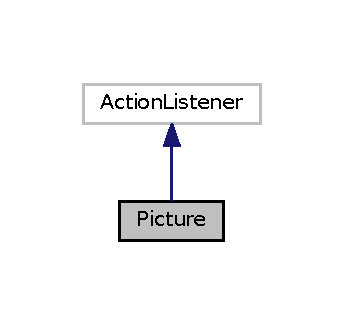
\includegraphics[width=165pt]{class_picture__inherit__graph}
\end{center}
\end{figure}


Collaboration diagram for Picture\+:
\nopagebreak
\begin{figure}[H]
\begin{center}
\leavevmode
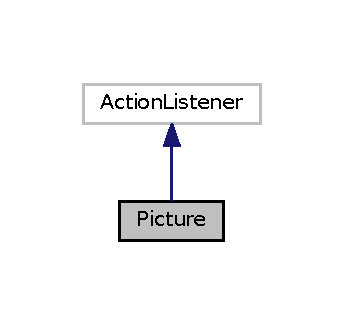
\includegraphics[width=165pt]{class_picture__coll__graph}
\end{center}
\end{figure}
\subsection*{Public Member Functions}
\begin{DoxyCompactItemize}
\item 
\hyperlink{class_picture_a07142473b84fdbdb91cb7025f7657027}{Picture} (int width, int height)
\item 
\hypertarget{class_picture_a4ecc0945f31dc27563195900e17c3a0a}{}{\bfseries Picture} (Buffered\+Image foto)\label{class_picture_a4ecc0945f31dc27563195900e17c3a0a}

\item 
\hyperlink{class_picture_ae1d35e34123c7658b727ca21bf79fec3}{Picture} (\hyperlink{class_picture}{Picture} picture)
\item 
\hyperlink{class_picture_a4ac461d816eb819710e51c139610ba68}{Picture} (String filename)
\item 
\hyperlink{class_picture_a1c4fa93e98dd54f073309a1e314b2ae9}{Picture} (File file)
\item 
J\+Label \hyperlink{class_picture_a23492bae036cfd015d79a0669f084bf5}{get\+J\+Label} ()
\item 
void \hyperlink{class_picture_a562666a5d8b36423da0aec5e92b9c078}{set\+Origin\+Upper\+Left} ()
\item 
void \hyperlink{class_picture_aa1513709f2fe6a54457294a5c271f9ef}{set\+Origin\+Lower\+Left} ()
\item 
void \hyperlink{class_picture_a7e2e47c6290831d31e9d0d6fae2e548d}{show} ()
\item 
int \hyperlink{class_picture_afca117450ab43ed8738b7ffa4fa6a2f7}{height} ()
\item 
int \hyperlink{class_picture_a4db9d5260d7c15056c85da767865b870}{width} ()
\item 
Color \hyperlink{class_picture_a8719d97ffafd78157647676cc4395f1d}{get} (int col, int row)
\item 
void \hyperlink{class_picture_a4e963f9fe2209d76d469428b458d6deb}{set} (int col, int row, Color color)
\item 
boolean \hyperlink{class_picture_af84a5e004ddf9d82121865290b049f97}{equals} (Object other)
\item 
int \hyperlink{class_picture_a768e1bf696a81fb573bd06c1a37df692}{hash\+Code} ()
\item 
void \hyperlink{class_picture_aba5d1df6955e8af12b889817fcab91af}{save} (String name)
\item 
void \hyperlink{class_picture_a0d547de85f185ad28e778ca0b108cf60}{save} (File file)
\item 
void \hyperlink{class_picture_addcd776af429ddb0593b63a6c8fb3253}{action\+Performed} (Action\+Event e)
\end{DoxyCompactItemize}
\subsection*{Static Public Member Functions}
\begin{DoxyCompactItemize}
\item 
static void \hyperlink{class_picture_ae507036e93b27aba4d1e06e44308798c}{main} (String\mbox{[}$\,$\mbox{]} args)
\end{DoxyCompactItemize}


\subsection{Detailed Description}
This class provides methods for manipulating individual pixels of an image. The original image can be read from a {\ttfamily .jpg}, {\ttfamily .gif}, or {\ttfamily .png} file or the user can create a blank image of a given size. This class includes methods for inputplaying the image in a window on the screen or saving it to a file. 

Pixel ({\itshape x}, {\itshape y}) is column {\itshape x} and row {\itshape y}. By default, the origin (0, 0) is upper left, which is a common convention in image processing. The method {\ttfamily \hyperlink{class_picture_aa1513709f2fe6a54457294a5c271f9ef}{set\+Origin\+Lower\+Left()}} change the origin to the lower left. 

For additional documentation, see \href{http://introcs.cs.princeton.edu/31datatype}{\tt Section 3.\+1} of {\itshape Introduction to Programming in Java\+: An Interinputciplinary Approach} by Robert Sedgewick and Kevin Wayne.

\begin{DoxyAuthor}{Author}
Robert Sedgewick 

Kevin Wayne 
\end{DoxyAuthor}


\subsection{Constructor \& Destructor Documentation}
\hypertarget{class_picture_a07142473b84fdbdb91cb7025f7657027}{}\index{Picture@{Picture}!Picture@{Picture}}
\index{Picture@{Picture}!Picture@{Picture}}
\subsubsection[{Picture}]{\setlength{\rightskip}{0pt plus 5cm}Picture.\+Picture (
\begin{DoxyParamCaption}
\item[{int}]{width, }
\item[{int}]{height}
\end{DoxyParamCaption}
)}\label{class_picture_a07142473b84fdbdb91cb7025f7657027}
Initializes a blank {\ttfamily width}-\/by-\/{\ttfamily height} picture, with {\ttfamily width} columns and {\ttfamily height} rows, where each pixel is black.


\begin{DoxyParams}{Parameters}
{\em width} & the width of the picture \\
\hline
{\em height} & the height of the picture \\
\hline
\end{DoxyParams}
\hypertarget{class_picture_ae1d35e34123c7658b727ca21bf79fec3}{}\index{Picture@{Picture}!Picture@{Picture}}
\index{Picture@{Picture}!Picture@{Picture}}
\subsubsection[{Picture}]{\setlength{\rightskip}{0pt plus 5cm}Picture.\+Picture (
\begin{DoxyParamCaption}
\item[{{\bf Picture}}]{picture}
\end{DoxyParamCaption}
)}\label{class_picture_ae1d35e34123c7658b727ca21bf79fec3}
Initializes a new picture that is a deep copy of the argument picture.


\begin{DoxyParams}{Parameters}
{\em picture} & the picture to copy \\
\hline
\end{DoxyParams}
\hypertarget{class_picture_a4ac461d816eb819710e51c139610ba68}{}\index{Picture@{Picture}!Picture@{Picture}}
\index{Picture@{Picture}!Picture@{Picture}}
\subsubsection[{Picture}]{\setlength{\rightskip}{0pt plus 5cm}Picture.\+Picture (
\begin{DoxyParamCaption}
\item[{String}]{filename}
\end{DoxyParamCaption}
)}\label{class_picture_a4ac461d816eb819710e51c139610ba68}
Initializes a picture by reading from a file or U\+R\+L.


\begin{DoxyParams}{Parameters}
{\em filename} & the name of the file (.png, .gif, or .jpg) or U\+R\+L. \\
\hline
\end{DoxyParams}
\hypertarget{class_picture_a1c4fa93e98dd54f073309a1e314b2ae9}{}\index{Picture@{Picture}!Picture@{Picture}}
\index{Picture@{Picture}!Picture@{Picture}}
\subsubsection[{Picture}]{\setlength{\rightskip}{0pt plus 5cm}Picture.\+Picture (
\begin{DoxyParamCaption}
\item[{File}]{file}
\end{DoxyParamCaption}
)}\label{class_picture_a1c4fa93e98dd54f073309a1e314b2ae9}
Initializes a picture by reading in a .png, .gif, or .jpg from a file.


\begin{DoxyParams}{Parameters}
{\em file} & the file \\
\hline
\end{DoxyParams}


\subsection{Member Function Documentation}
\hypertarget{class_picture_addcd776af429ddb0593b63a6c8fb3253}{}\index{Picture@{Picture}!action\+Performed@{action\+Performed}}
\index{action\+Performed@{action\+Performed}!Picture@{Picture}}
\subsubsection[{action\+Performed}]{\setlength{\rightskip}{0pt plus 5cm}void Picture.\+action\+Performed (
\begin{DoxyParamCaption}
\item[{Action\+Event}]{e}
\end{DoxyParamCaption}
)}\label{class_picture_addcd776af429ddb0593b63a6c8fb3253}
Opens a save dialog box when the user selects \char`\"{}\+Save As\char`\"{} from the menu. \hypertarget{class_picture_af84a5e004ddf9d82121865290b049f97}{}\index{Picture@{Picture}!equals@{equals}}
\index{equals@{equals}!Picture@{Picture}}
\subsubsection[{equals}]{\setlength{\rightskip}{0pt plus 5cm}boolean Picture.\+equals (
\begin{DoxyParamCaption}
\item[{Object}]{other}
\end{DoxyParamCaption}
)}\label{class_picture_af84a5e004ddf9d82121865290b049f97}
Returns true if this picture is equal to the argument picture.


\begin{DoxyParams}{Parameters}
{\em other} & the other picture \\
\hline
\end{DoxyParams}
\begin{DoxyReturn}{Returns}
{\ttfamily true} if this picture is the same dimension as {\ttfamily other} and if all pixels have the same color; {\ttfamily false} otherwise 
\end{DoxyReturn}
\hypertarget{class_picture_a8719d97ffafd78157647676cc4395f1d}{}\index{Picture@{Picture}!get@{get}}
\index{get@{get}!Picture@{Picture}}
\subsubsection[{get}]{\setlength{\rightskip}{0pt plus 5cm}Color Picture.\+get (
\begin{DoxyParamCaption}
\item[{int}]{col, }
\item[{int}]{row}
\end{DoxyParamCaption}
)}\label{class_picture_a8719d97ffafd78157647676cc4395f1d}
Returns the color of pixel ({\ttfamily col}, {\ttfamily row}).


\begin{DoxyParams}{Parameters}
{\em col} & the column index \\
\hline
{\em row} & the row index \\
\hline
\end{DoxyParams}
\begin{DoxyReturn}{Returns}
the color of pixel ({\ttfamily col}, {\ttfamily row}) 
\end{DoxyReturn}

\begin{DoxyExceptions}{Exceptions}
{\em Index\+Out\+Of\+Bounds\+Exception} & unless both 0 {$\le$} {\ttfamily col} $<$ {\ttfamily width} and 0 {$\le$} {\ttfamily row} $<$ {\ttfamily height} \\
\hline
\end{DoxyExceptions}
\hypertarget{class_picture_a23492bae036cfd015d79a0669f084bf5}{}\index{Picture@{Picture}!get\+J\+Label@{get\+J\+Label}}
\index{get\+J\+Label@{get\+J\+Label}!Picture@{Picture}}
\subsubsection[{get\+J\+Label}]{\setlength{\rightskip}{0pt plus 5cm}J\+Label Picture.\+get\+J\+Label (
\begin{DoxyParamCaption}
{}
\end{DoxyParamCaption}
)}\label{class_picture_a23492bae036cfd015d79a0669f084bf5}
Returns a J\+Label containing this picture, for embedding in a J\+Panel, J\+Frame or other G\+U\+I widget.

\begin{DoxyReturn}{Returns}
the {\ttfamily J\+Label} 
\end{DoxyReturn}
\hypertarget{class_picture_a768e1bf696a81fb573bd06c1a37df692}{}\index{Picture@{Picture}!hash\+Code@{hash\+Code}}
\index{hash\+Code@{hash\+Code}!Picture@{Picture}}
\subsubsection[{hash\+Code}]{\setlength{\rightskip}{0pt plus 5cm}int Picture.\+hash\+Code (
\begin{DoxyParamCaption}
{}
\end{DoxyParamCaption}
)}\label{class_picture_a768e1bf696a81fb573bd06c1a37df692}
This operation is not supported because pictures are mutable.

\begin{DoxyReturn}{Returns}
does not return a value 
\end{DoxyReturn}

\begin{DoxyExceptions}{Exceptions}
{\em Unsupported\+Operation\+Exception} & if called \\
\hline
\end{DoxyExceptions}
\hypertarget{class_picture_afca117450ab43ed8738b7ffa4fa6a2f7}{}\index{Picture@{Picture}!height@{height}}
\index{height@{height}!Picture@{Picture}}
\subsubsection[{height}]{\setlength{\rightskip}{0pt plus 5cm}int Picture.\+height (
\begin{DoxyParamCaption}
{}
\end{DoxyParamCaption}
)}\label{class_picture_afca117450ab43ed8738b7ffa4fa6a2f7}
Returns the height of the picture.

\begin{DoxyReturn}{Returns}
the height of the picture (in pixels) 
\end{DoxyReturn}
\hypertarget{class_picture_ae507036e93b27aba4d1e06e44308798c}{}\index{Picture@{Picture}!main@{main}}
\index{main@{main}!Picture@{Picture}}
\subsubsection[{main}]{\setlength{\rightskip}{0pt plus 5cm}static void Picture.\+main (
\begin{DoxyParamCaption}
\item[{String\mbox{[}$\,$\mbox{]}}]{args}
\end{DoxyParamCaption}
)\hspace{0.3cm}{\ttfamily [static]}}\label{class_picture_ae507036e93b27aba4d1e06e44308798c}
Unit tests this {\ttfamily \hyperlink{class_picture}{Picture}} data type. Reads a picture specified by the command-\/line argument, and shows it in a window on the screen. \hypertarget{class_picture_aba5d1df6955e8af12b889817fcab91af}{}\index{Picture@{Picture}!save@{save}}
\index{save@{save}!Picture@{Picture}}
\subsubsection[{save}]{\setlength{\rightskip}{0pt plus 5cm}void Picture.\+save (
\begin{DoxyParamCaption}
\item[{String}]{name}
\end{DoxyParamCaption}
)}\label{class_picture_aba5d1df6955e8af12b889817fcab91af}
Saves the picture to a file in a standard image format. The filetype must be .png or .jpg.


\begin{DoxyParams}{Parameters}
{\em name} & the name of the file \\
\hline
\end{DoxyParams}
\hypertarget{class_picture_a0d547de85f185ad28e778ca0b108cf60}{}\index{Picture@{Picture}!save@{save}}
\index{save@{save}!Picture@{Picture}}
\subsubsection[{save}]{\setlength{\rightskip}{0pt plus 5cm}void Picture.\+save (
\begin{DoxyParamCaption}
\item[{File}]{file}
\end{DoxyParamCaption}
)}\label{class_picture_a0d547de85f185ad28e778ca0b108cf60}
Saves the picture to a file in a P\+N\+G or J\+P\+E\+G image format.


\begin{DoxyParams}{Parameters}
{\em file} & the file \\
\hline
\end{DoxyParams}
\hypertarget{class_picture_a4e963f9fe2209d76d469428b458d6deb}{}\index{Picture@{Picture}!set@{set}}
\index{set@{set}!Picture@{Picture}}
\subsubsection[{set}]{\setlength{\rightskip}{0pt plus 5cm}void Picture.\+set (
\begin{DoxyParamCaption}
\item[{int}]{col, }
\item[{int}]{row, }
\item[{Color}]{color}
\end{DoxyParamCaption}
)}\label{class_picture_a4e963f9fe2209d76d469428b458d6deb}
Sets the color of pixel ({\ttfamily col}, {\ttfamily row}) to given color.


\begin{DoxyParams}{Parameters}
{\em col} & the column index \\
\hline
{\em row} & the row index \\
\hline
{\em color} & the color \\
\hline
\end{DoxyParams}

\begin{DoxyExceptions}{Exceptions}
{\em Index\+Out\+Of\+Bounds\+Exception} & unless both 0 {$\le$} {\ttfamily col} $<$ {\ttfamily width} and 0 {$\le$} {\ttfamily row} $<$ {\ttfamily height} \\
\hline
{\em Null\+Pointer\+Exception} & if {\ttfamily color} is {\ttfamily null} \\
\hline
\end{DoxyExceptions}
\hypertarget{class_picture_aa1513709f2fe6a54457294a5c271f9ef}{}\index{Picture@{Picture}!set\+Origin\+Lower\+Left@{set\+Origin\+Lower\+Left}}
\index{set\+Origin\+Lower\+Left@{set\+Origin\+Lower\+Left}!Picture@{Picture}}
\subsubsection[{set\+Origin\+Lower\+Left}]{\setlength{\rightskip}{0pt plus 5cm}void Picture.\+set\+Origin\+Lower\+Left (
\begin{DoxyParamCaption}
{}
\end{DoxyParamCaption}
)}\label{class_picture_aa1513709f2fe6a54457294a5c271f9ef}
Sets the origin to be the lower left pixel. \hypertarget{class_picture_a562666a5d8b36423da0aec5e92b9c078}{}\index{Picture@{Picture}!set\+Origin\+Upper\+Left@{set\+Origin\+Upper\+Left}}
\index{set\+Origin\+Upper\+Left@{set\+Origin\+Upper\+Left}!Picture@{Picture}}
\subsubsection[{set\+Origin\+Upper\+Left}]{\setlength{\rightskip}{0pt plus 5cm}void Picture.\+set\+Origin\+Upper\+Left (
\begin{DoxyParamCaption}
{}
\end{DoxyParamCaption}
)}\label{class_picture_a562666a5d8b36423da0aec5e92b9c078}
Sets the origin to be the upper left pixel. This is the default. \hypertarget{class_picture_a7e2e47c6290831d31e9d0d6fae2e548d}{}\index{Picture@{Picture}!show@{show}}
\index{show@{show}!Picture@{Picture}}
\subsubsection[{show}]{\setlength{\rightskip}{0pt plus 5cm}void Picture.\+show (
\begin{DoxyParamCaption}
{}
\end{DoxyParamCaption}
)}\label{class_picture_a7e2e47c6290831d31e9d0d6fae2e548d}
inputplays the picture in a window on the screen. \hypertarget{class_picture_a4db9d5260d7c15056c85da767865b870}{}\index{Picture@{Picture}!width@{width}}
\index{width@{width}!Picture@{Picture}}
\subsubsection[{width}]{\setlength{\rightskip}{0pt plus 5cm}int Picture.\+width (
\begin{DoxyParamCaption}
{}
\end{DoxyParamCaption}
)}\label{class_picture_a4db9d5260d7c15056c85da767865b870}
Returns the width of the picture.

\begin{DoxyReturn}{Returns}
the width of the picture (in pixels) 
\end{DoxyReturn}


The documentation for this class was generated from the following file\+:\begin{DoxyCompactItemize}
\item 
Picture.\+java\end{DoxyCompactItemize}

\hypertarget{class_server}{}\section{Server Class Reference}
\label{class_server}\index{Server@{Server}}


Clase que contiene el main que inicia el servidor y controla los threads que reciben las imágenes.  




Inheritance diagram for Server\+:
\nopagebreak
\begin{figure}[H]
\begin{center}
\leavevmode
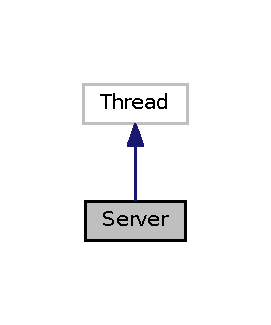
\includegraphics[width=130pt]{class_server__inherit__graph}
\end{center}
\end{figure}


Collaboration diagram for Server\+:
\nopagebreak
\begin{figure}[H]
\begin{center}
\leavevmode
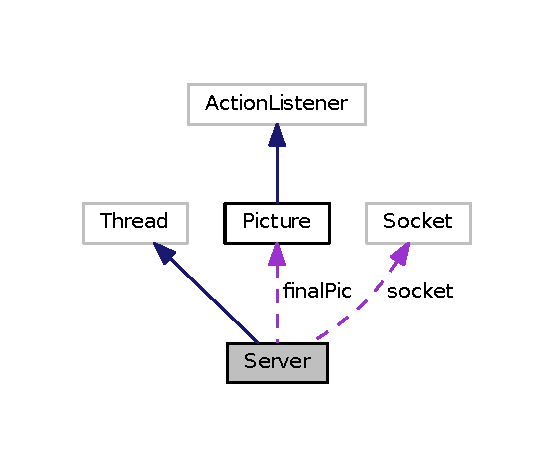
\includegraphics[width=266pt]{class_server__coll__graph}
\end{center}
\end{figure}
\subsection*{Public Member Functions}
\begin{DoxyCompactItemize}
\item 
\hyperlink{class_server_a906efb564818baa15e207fc6d4b26b3f}{Server} (Socket socket, int iterations, \hyperlink{class_iteration}{Iteration} iteration, \hyperlink{class_picture}{Picture} img)
\begin{DoxyCompactList}\small\item\em Método constructor de la clase. \end{DoxyCompactList}\item 
void \hyperlink{class_server_a2f44e49f6ef4699f17b88314bc2104c6}{desconnectar} ()
\begin{DoxyCompactList}\small\item\em Método que realiza la desconexión. \end{DoxyCompactList}\item 
void \hyperlink{class_server_ace0ce586af36c8024040a43db4054ab7}{run} ()
\begin{DoxyCompactList}\small\item\em Método run que gestiona los threads en el servidor. \end{DoxyCompactList}\end{DoxyCompactItemize}
\subsection*{Static Public Member Functions}
\begin{DoxyCompactItemize}
\item 
static void \hyperlink{class_server_ad90c92078da8d9c8a084e7cbc6cff4af}{main} (String args\mbox{[}$\,$\mbox{]})
\begin{DoxyCompactList}\small\item\em Método main de la clase. \end{DoxyCompactList}\end{DoxyCompactItemize}


\subsection{Detailed Description}
Clase que contiene el main que inicia el servidor y controla los threads que reciben las imágenes. 

\begin{DoxyAuthor}{Author}
Nara, Javier, Esteban 
\end{DoxyAuthor}


\subsection{Constructor \& Destructor Documentation}
\hypertarget{class_server_a906efb564818baa15e207fc6d4b26b3f}{}\index{Server@{Server}!Server@{Server}}
\index{Server@{Server}!Server@{Server}}
\subsubsection[{Server}]{\setlength{\rightskip}{0pt plus 5cm}Server.\+Server (
\begin{DoxyParamCaption}
\item[{Socket}]{socket, }
\item[{int}]{iterations, }
\item[{{\bf Iteration}}]{iteration, }
\item[{{\bf Picture}}]{img}
\end{DoxyParamCaption}
)}\label{class_server_a906efb564818baa15e207fc6d4b26b3f}


Método constructor de la clase. 

\begin{DoxyAuthor}{Author}
Nara, Javier, Esteban 
\end{DoxyAuthor}

\begin{DoxyParams}{Parameters}
{\em socket} & \+: Socket \\
\hline
{\em iterations} & \+: Número de iteraciones necesarias para rellenar la foto \\
\hline
{\em iteration} & \+: Iteración recibida \\
\hline
{\em img} & \+: Imagen actual que se aplicará \\
\hline
\end{DoxyParams}


\subsection{Member Function Documentation}
\hypertarget{class_server_a2f44e49f6ef4699f17b88314bc2104c6}{}\index{Server@{Server}!desconnectar@{desconnectar}}
\index{desconnectar@{desconnectar}!Server@{Server}}
\subsubsection[{desconnectar}]{\setlength{\rightskip}{0pt plus 5cm}void Server.\+desconnectar (
\begin{DoxyParamCaption}
{}
\end{DoxyParamCaption}
)}\label{class_server_a2f44e49f6ef4699f17b88314bc2104c6}


Método que realiza la desconexión. 

\begin{DoxyAuthor}{Author}
Nara, Javier, Esteban 
\end{DoxyAuthor}
\hypertarget{class_server_ad90c92078da8d9c8a084e7cbc6cff4af}{}\index{Server@{Server}!main@{main}}
\index{main@{main}!Server@{Server}}
\subsubsection[{main}]{\setlength{\rightskip}{0pt plus 5cm}static void Server.\+main (
\begin{DoxyParamCaption}
\item[{String}]{args\mbox{[}$\,$\mbox{]}}
\end{DoxyParamCaption}
)\hspace{0.3cm}{\ttfamily [static]}}\label{class_server_ad90c92078da8d9c8a084e7cbc6cff4af}


Método main de la clase. 

\begin{DoxyAuthor}{Author}
Nara, Javier, Esteban 
\end{DoxyAuthor}

\begin{DoxyParams}{Parameters}
{\em args\mbox{[}$\,$\mbox{]}} & \+: Array de argumentos pasados como parámetros \\
\hline
\end{DoxyParams}
\hypertarget{class_server_ace0ce586af36c8024040a43db4054ab7}{}\index{Server@{Server}!run@{run}}
\index{run@{run}!Server@{Server}}
\subsubsection[{run}]{\setlength{\rightskip}{0pt plus 5cm}void Server.\+run (
\begin{DoxyParamCaption}
{}
\end{DoxyParamCaption}
)}\label{class_server_ace0ce586af36c8024040a43db4054ab7}


Método run que gestiona los threads en el servidor. 

\begin{DoxyAuthor}{Author}
Nara, Javier, Esteban 
\end{DoxyAuthor}


The documentation for this class was generated from the following file\+:\begin{DoxyCompactItemize}
\item 
Server.\+java\end{DoxyCompactItemize}

%--- End generated contents ---

% Index
\backmatter
\newpage
\phantomsection
\clearemptydoublepage
\addcontentsline{toc}{chapter}{Index}
\printindex

\end{document}
